\documentclass{article}

\usepackage{graphicx}
\usepackage[legalpaper, portrait, margin=1in]{geometry}
\usepackage{xcolor}
\usepackage{color,soul}
\newcommand\todo[1]{\textcolor{red}{#1}}

\usepackage{subcaption}


\title{Supervised Learning - CS7641 Fall 2021}
\author{Huifu Tian}
\begin{document}
\maketitle


In this assignment, I will use the Polish companies bankruptcy data set and the MNIST handwritten digits data set to compare various supervised learning algorithms. All of the analysis was done using the scikit-learn library compatible with Python 3.



\section{Polish Data}

\subsection{Data Overview}
This dataset is a collection of Polish companies spanning 2007-2013. The dataset contains a total of roughly 700 bankrupt companies corresponding to 2400 financial reports in the period between 2007 and 2013. The data is separated into five datasets - 1stYear, 2ndYear, 3rdYear, 4thYear, 5thYear. Each row in every data set contains the financial report of one company in a single year. \newline

- 1stYear: 7027 surveyed companies in 2007, 271 of which went bankrupt by the start of 2013

- 2ndYear: 10173 surveyed companies in 2008, 400 of which went bankrupt by the start of 2013

- 3rdYear: 10503 surveyed companies in 2009, 495 of which went bankrupt by the start of 2013

- 4thYear: 9792 surveyed companies in 2010, 515 of which went bankrupt by the start of 2013

- 5thYear: 5910 surveyed companies in 2011, 410 of which went bankrupt by the start of 2013\newline


The attributes are are shown in Table 1. \newline

The output consists of one column where 1 means bankruptcy and 0 means non-bankruptcy. \newline

\todo{add more stats exploring the data such as autocorrelations, class sizes, etc}

\begin{table}
	Table 1: Polish companies bankruptcy data attributes
	\centering
	\begin{tabular}{| l | l |}
		\hline
		X1 net profit / total assets                                                                                                                                       & {X33 operating expenses / short-term liabilities}                                                                                      \\ \hline
		X2 total liabilities / total assets                                                                                                                                & {X34 operating expenses / total liabilities}                                                                                           \\ \hline
		X3 working capital / total assets                                                                                                                                  & X35 profit on sales / total assets                                                                                                           \\ \hline
		X4 current assets / short-term liabilities                                                                                                                         & X36 total sales / total assets                                                                                                               \\ \hline
		\begin{tabular}[c]{@{}l@{}}X5 [(cash + short-term securities + receivables \\- short-term liabilities) \\/ (operating expenses - depreciation)] * 365\end{tabular} & X37 (current assets - inventories) / long-term liabilities                                                                                   \\ \hline
		X6 retained earnings / total assets                                                                                                                                & X38 constant capital / total assets                                                                                                          \\ \hline
		X7 EBIT / total assets                                                                                                                                             & X39 profit on sales / sales                                                                                                                  \\ \hline
		X8 book value of equity / total liabilities                                                                                                                        & \begin{tabular}[c]{@{}l@{}}X40 (current assets - inventory - receivables) \\/ short-term liabilities\end{tabular}                            
		\\ \hline
		X9 sales / total assets                                                                                                                                            & \begin{tabular}[c]{@{}l@{}}X41 total liabilities \\/ ((profit on operating activities + depreciation) \\$\times$ (12/365))\end{tabular}               
		\\ \hline
		X10 equity / total assets                                                                                                                                          & X42 profit on operating activities / sales                                                                                                   \\ \hline
		\begin{tabular}[c]{@{}l@{}}X11 (gross profit + extraordinary items \\+ financial expenses) \\/ total assets\end{tabular}                                           & X43 rotation receivables + inventory turnover in days                                                                                        \\ \hline
		X12 gross profit / short-term liabilities                                                                                                                          & X44 (receivables * 365) / sales                                                                                                              \\ \hline
		X13 (gross profit + depreciation) / sales                                                                                                                          & X45 net profit / inventory                                                                                                                   \\ \hline
		X14 (gross profit + interest) / total assets                                                                                                                       & X46 (current assets - inventory) / short-term liabilities                                                                                    \\ \hline
		\begin{tabular}[c]{@{}l@{}}X15 (total liabilities * 365) 
		\\	/ (gross profit + depreciation)         \end{tabular}                        
		                                                                                             & X47 (inventory * 365) / cost of products sold                                                                                                \\ \hline
		X16 (gross profit + depreciation) / total liabilities                                                                                                              & \begin{tabular}[c]{@{}l@{}}X48 EBITDA / total assets\end{tabular}                          
		\\ \hline
		X17 total assets / total liabilities                                                                                                                               & \begin{tabular}[c]{@{}l@{}}X49 EBITDA / sales\end{tabular}                                 
		\\ \hline
		X18 gross profit / total assets                                                                                                                                    & X50 current assets / total liabilities                                                                                                       \\ \hline
		X19 gross profit / sales                                                                                                                                           & X51 short-term liabilities / total assets                                                                                                    \\ \hline
		X20 (inventory * 365) / sales                                                                                                                                      & X52 (short-term liabilities * 365) / cost of products sold)                                                                                  \\
		X21 sales (n) / sales (n-1)                                                                                                                                        & X53 equity / fixed assets                                                                                                                    \\ \hline
		X22 profit on operating activities / total assets                                                                                                                  & X54 constant capital / fixed assets                                                                                                          \\ \hline
		{X23 net profit / sales}                                                                                                                                     & X55 working capital                                                                                                                          \\ \hline
		X24 gross profit (in 3 years) / total assets                                                                                                                       & X56 (sales - cost of products sold) / sales                                                                                                  \\ \hline
		X25 (equity - share capital) / total assets                                                                                                                        & \begin{tabular}[c]{@{}l@{}}X57 (current assets - inventory - short-term liabilities) \\/ (sales - gross profit - depreciation)\end{tabular}  
		\\ \hline
		X26 (net profit + depreciation) / total liabilities                                                                                                                & X58 total costs /total sales                                                                                                                 \\ \hline
		\begin{tabular}[c]{@{}l@{}}X27 profit on operating activities \\/ financial expenses \end{tabular}
        & X59 long-term liabilities / equity                                                                                                           \\ \hline
		X28 working capital / fixed assets                                                                                                                                 & X60 sales / inventory                                                                                                                        \\ \hline
		X29 logarithm of total assets                                                                                                                                      & X61 sales / receivables                                                                                                                      \\ \hline
		X30 (total liabilities - cash) / sales                                                                                                                             & X62 (short-term liabilities *365) / sales                                                                                                    \\ \hline
		X31 (gross profit + interest) / sales                                                                                                                              & X63 sales / short-term liabilities                                                                                                           \\ \hline
		X32 (current liabilities * 365) / cost of products sold                                                                                                            & X64 sales / fixed assets
		\\
		\hline                                                                                                    
	\end{tabular}
\end{table}

\subsection{Preprocessing}

Minimal preprocessing was done to keep the focus on analysis. I combined all of the data sets to form a new dataset of over 43000 rows, which may introduce oversampling bias since it's not guaranteed that each company that is marked with a bankruptcy status=1 only shows up once across the 5 data sets. \todo{is it called oversampling bias?} All of the infrequent NaNs in the attribute columns are replaced with 0's. (There are no NaNs in the output column.) Finally, I divide the data into 70\% train and 30\% test sets while applying stratification to ensure uniform distribution of classes between the two groups. 


\subsection{Decision Tree}

\subsubsection*{Baseline model}

The baseline model uses sklearn's DecisionTreeClassifier class and is trained with unlimited tree depth and the Gini measure of impurity. The error measure that we care about depends largely on the reason we are doing this study and whether or not our data is imbalanced. If the goal is to predict with high confidence that a company predicted to go bankrupt will actually go bankrupt (i.e. to construct a portfolio of assets to short), then we might care a lot about precision. On the other hand, if we care about finding all the companies that might go bankrupt, then we should use recall, or balanced accuracy, which is the mean of recall on both classes. The other observation is that our data is imbalanced: about 4.5\% of the data falls in the minority (bankrupt) class. Table 2 shows the mean metric scores from fitting the classifier on the training data and scoring on the test data with various undersampling ratios across 20 iterations of random sampling from the majority class.

\begin{table}
	\centering
	Table 2: Mean Decision Tree Classifier Baseline Scores with Undersampling
	\begin{tabular}{ l l l l l }
		\hline
		Metric & No Undersampling\footnote[1] & 3:1 \footnote[2] & 2:1 & 1:1 \\
		\hline
		Accuracy & 0.95 & 0.83 & 0.81 & 0.78 \\
		F1 & 0.48 & 0.67 & 0.71 & 0.78 \\
		Precision & 0.46 & 0.66 & 0.71 & 0.78 \\
		Recall & 0.50 & 0.68 & 0.72 & 0.79 \\
		Balanced accuracy & 0.73 & 0.78 & 0.78 & 0.78 \\
		Fitted tree depth & 33 & 24.25 & 22.8 & 19.65\\
		\hline 
		

	\end{tabular}
	\footnotetext[1]{Only one iteration of fitting}
	\footnotetext[2]{ratio of the post-undersampled majority to minority class}
\end{table}

Before tuning the model, it's worth noting that the decision tree classifier exhibits the general behavior one tends to see with imbalanced data sets, namely that the classifier prefers to minimize error for the majority class at the expense of the minority class. As the sample rebalancing approaches parity between both classes (shown by the progression from 3:1 to 1:1 ratio), precision, recall, and accuracy of the minority class are all improved. As a bonus, fitted tree depth also becomes smaller, which is preferred because we like simpler models over more complex models. \newline

\subsubsection*{Model Tuning}
\subsubsection*{Impurity}
Table 3 shows the same analysis as Table 2 using the entropy instead of gini as the impurity measure. The reuslts are similar. Since the entropy measure takes longer to calculate due to logs in the measure and it doesn't offer significant improvements, we can stick to using gini measure for the rest of the analysis.

\begin{table}
	\centering
	Table 3: Mean Decision Tree Classifier Baseline Scores with Undersampling using Entropy
	\begin{tabular}{ l l l l l }
		\hline
		Metric & No Undersampling\footnote[1] & 3:1 \footnote[2] & 2:1 & 1:1 \\
		\hline
		Accuracy & 0.95 & 0.84 & 0.81 & 0.79 \\
		F1 & 0.52 & 0.68 & 0.71 & 0.79 \\
		Precision & 0.51 & 0.68 & 0.71 & 0.78 \\
		Recall & 0.50 & 0.69 & 0.72 & 0.79 \\
		Balanced accuracy & 0.75 & 0.79 & 0.79 & 0.79 \\
		Fitted tree depth & 26 & 21.8 & 20.9 & 19.75\\
		\hline 
		
		
	\end{tabular}
	\footnotetext[1]{Only one iteration of fitting}
	\footnotetext[2]{ratio of the post-undersampled majority to minority class}
\end{table}

\subsubsection*{Max Tree Depth}
Without bounding max tree depth, the baseline model will fit the data to a tree with average depth of 19.65 (Table 2) using 1:1 rebalancing across 20 random samplings across the majority class. To determine the ideal max tree depth, I use a modified version of the Stratified K Folds validation algorithm. Rather than selecting k folds to split one set of the post-undersampled training data into a train and validation set, I select 2 folds across k sets of training data. The reason for this modification is that I'm undersampling the majority class. To reduce the variance of results across multiple trials as much as possible, hence k folds, it makes more sense to randomly pick from a much bigger pool of data than to undersample first then pick from a smaller pool of data. The results are shown in Figure 1.

\begin{figure}
	\centering
	Figure 1: Validation Curve: Max Tree Depth
	\makebox[\textwidth]{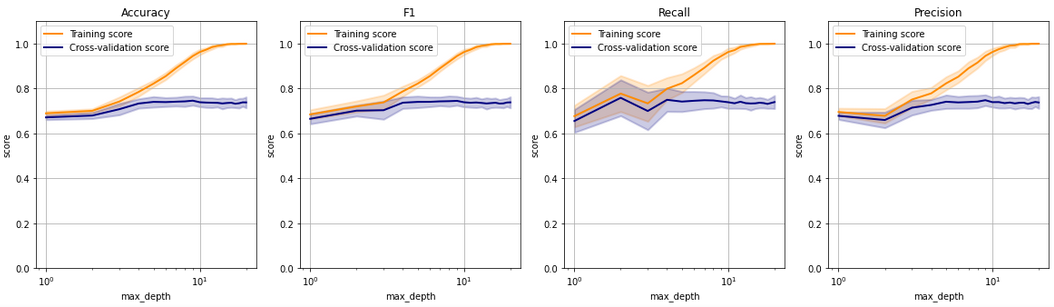
\includegraphics[width=\textwidth]{poland_decision_max_tree_depth_validation.png}}
\end{figure}

The validation curves in Figure 1 show increasing training scores in general. The testing scores are increasing at first before tapering off slightly as max\_depth becomes large. The optimal max\_depth value is such that there is no overfitting or underfitting. That point occurs when the test score reaches its highest point before gradually tapering off. The maximum values for all four scores are shown in the table below.

\begin{center}
	Table 4: Optimal Max Tree Depth
	\begin{tabular}{ l l l l l }
		\hline
		Metric & Max Tree Depth & Min Samples Split & Min Samples Leaf & haha \\
		\hline
		Accuracy & 0.95 & 0.84 & 0.81 & 0.79 \\
		F1 & 0.52 & 0.68 & 0.71 & 0.79 \\
		Precision & 0.51 & 0.68 & 0.71 & 0.78 \\
		Recall & 0.50 & 0.69 & 0.72 & 0.79 \\
		Balanced accuracy & 0.75 & 0.79 & 0.79 & 0.79 \\
		Fitted tree depth & 26 & 21.8 & 20.9 & 19.75\\
		\hline 
		
		
	\end{tabular}
	\footnotetext[1]{Only one iteration of fitting}
	\footnotetext[2]{ratio of the post-undersampled majority to minority class}
\end{center}

\begin{figure}
	\centering
	Figure 2: Validation curve: Min Samples Split
	\makebox[\textwidth]{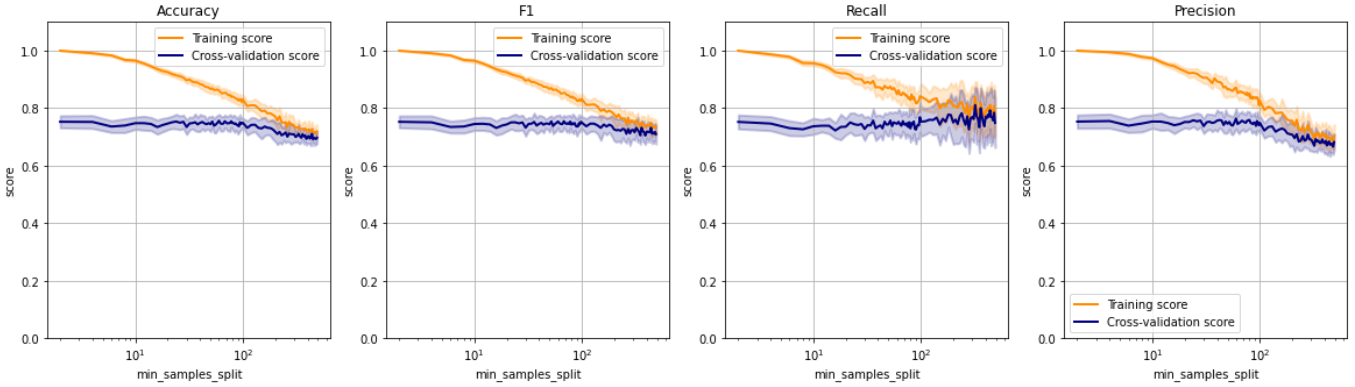
\includegraphics[width=\textwidth]{poland_decision_min_samples_split.png}}
\end{figure}

\subsubsection*{Min Samples Split}
Another hyperparameter we can use to tune the model is the minimum number of samples required for a node before the node can be further split. I repeat the same procedure with the modified Stratified K Folds with and without controlling for max tree depth. The validation curves for minimum samples split while setting max tree depth to the optimal value of 9 are shown in Figure 2. Both sets of validation curves (setting and not setting max depth - not shown) look similar. Metric scores on the training set are decreasing from 2 to 100 are decreasing while the scores on the validation set are flat. It's possible to find an ``optimal'' $n$ such that test scores are maximized but additional studies must be done to validate that the maximum value at the ``optimal'' $n$ is statistically different from another value. \todo{do this analysis?}

\subsubsection*{Cost Complexity Pruning}
The last parameter I will tune is the cost complexity pruning alpha. This parameter reduces the weak links in the tree by removing those nodes and all of their child trees. The alphas are a regularization parameter that penalizes the number of leaves in the fitted tree. I run cost complexity pruning after setting max\_depth to the optimal number. The result (not shown \todo{show if there's space}) indicate that doing post pruning does not improve accuracy of model when evaluated on the test set. 

\subsection*{Learning Curves}

To understand whether our model is overfitting or underfitting, I make two learning curves: one without restrictions, one with max tree depth. In the case without setting max\_depth, the training accuracy scores stay at roughly 100\%. This shows that the model was likely too complex and fit the training model perfectly. The idea that this model is overfitting the data is also supported by the fact that the validation scores remain flat, meaning that the model is unable to generalize. Once I introduce max\_depth, the training model's accuracy scores start to decrease as we limit the model's complexity. The result is that a simpler model does better at generalization, which is shown by the much improved scores on the test data. There is still a gap between the training curve and the validation curve at the 2000th sample, which means that further limiting of the model's complexity may improve the validation score. Also, validation scores are still in the middle of improving at the 2000th sample, which implies that having more samples would improve the model's ability to fit the data. \todo{discuss variance and bias}

\begin{figure}
\centering
Figure 3
\begin{subfigure}{.5\textwidth}
\centering
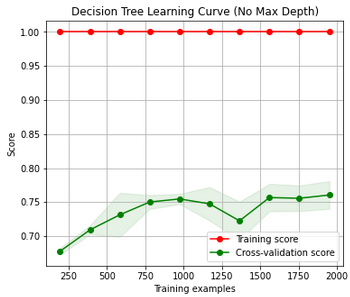
\includegraphics[width=\linewidth]{poland_decision_learning_curve_without_max_depth.png}

\end{subfigure}%
\begin{subfigure}{.5\textwidth}
\centering
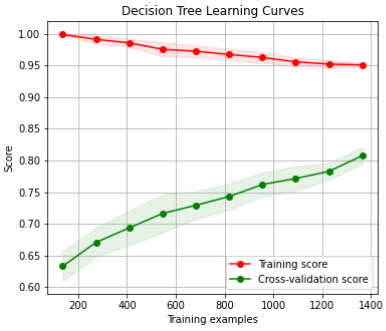
\includegraphics[width=\linewidth]{poland_decision_learning_curve_with_max_depth.png}

\end{subfigure}
\label{fig:test}
\end{figure}

\subsubsection*{Final model and performance}

The model with max\_depth set to 9 yields is run 20 times using 1:1 balanced sampling between the two classes, each time picking a 70\% training and 30\% testing set. The mean accuracy across the 20 iterations is 0.79. \todo{Show in final summary table}

\subsection{Neural Network}

\subsubsection*{Baseline model}

Similar to the decision trees, I use the full data set which combines all five data sets and use a 70-30 train-test split. Table 5 column 1 shows that attempting to use neural network to fit the data without first normalizing the inputs leads to non-convergeance. Column 2 normalizes all of the features by removing the mean and scaling to unit variance. Columns 3 and 4 show the results with 3:1 and 1:1 majority to minority class undersampling. With columns 3 and 4, I the scores displayed in the second part of the table have been averaged across 20 independent iterations. As we move from the full data set to a 1:1 rebalanced data set, accuracy decreases while f1, precision, recall, and balanced accuracy all increase. It can be seen that neural networks suffer from the same majority class bias as decision trees: accuracy is maximized by focusing on fitting the model to the majority class while neglecting the minority class. Intuitively, that makes sense, the algorithm strives to maximize accuracy. High accuracy can only be achieved by catering more attention to the majority class. 

\subsubsection*{Model Tuning}
\subsubsection*{Number of Hidden Nodes}





\begin{table}

	\centering
	Table 5: Neural Network Parameters and Results\\
	\begin{tabular}{ l l l l l }
		\hline
		Parameter & 1 & 2 & 3 & 4\\
		\hline
		solver & sgd & sgd & sgd & sgd\\
		activation & relu & relu & relu & relu\\
		alpha & 0.01 & 0.01 & 0.01 & 0.01\\
		hidden\_layer\_sizes & (30,) & (30,) & (30,) & (30,)\\
		max\_iter & 1000 & 1000 & 1000 & 1000\\
		learning\_rate & constant & constant & constant & constant \\
		learning\_rate\_init & 0.001 & 0.001 & 0.001 & 0.001 \\
		momentum & 0.9 & 0.9 & 0.9 & 0.9 \\
		Normalized? & No & \hl{Yes} & Yes & Yes\\
		Undersampled? & No & No & \hl{3:1} & \hl{1:1}\\
		\hline
		Results & & & & \\
		\hline
		Accuracy & & 0.952 & 0.757 & 0.643 \\
		F1 &  & 0.003 & 0.151 & 0.635 \\
		Precision & & 0.333 & 0.597 & 0.648  \\
		Recall & & 0.002 & 0.089 & 0.624 \\
		Balanced accuracy & & 0.501 & 0.535 & 0.643 \\
	
		\hline 
	\end{tabular}
\end{table}

\end{document}